%%%%%%%%%%%%%%%%%%%%%%%%%%%%%%%%%%%%%%%%%%%%%%%%%%%%%%%%%%%%%%%%%%%%%%%%%%%%%%%
% CHAPTER 4: Results and Analysis
%       DUE: October 15, 2025
%     PAGES: 25-30
%%%%%%%%%%%%%%%%%%%%%%%%%%%%%%%%%%%%%%%%%%%%%%%%%%%%%%%%%%%%%%%%%%%%%%%%%%%%%%%
\chapter{Results and Analysis}
\label{chap:results}

\section{Chapter Overview}
\label{sec:results_overview}

This chapter presents the empirical results obtained from the experiments detailed in \cref{chap:methodology}. The findings are organized to systematically address the research questions and hypotheses concerning the use of Large Language Models (LLMs) to construct knowledge graphs (KGs) for document validation. The core of this research explores a framework built on three dimensions of validation: correctness, completeness, and consistency.

The chapter begins by detailing the experimental setup, including the computational environment, datasets, and the methodology for establishing ground truth. It then presents the outcomes of preliminary experiments focused on hyperparameter tuning, which established the optimal configuration for the main experimental runs.

The main results are presented in three parts, structured according to the evaluation framework:
\begin{enumerate}
    \item \textbf{Knowledge Graph Fit Assessment:} An evaluation of the quality, traceability, and structural integrity of the generated KGs.
    \item \textbf{Suitability for Consistency and Completeness (C\&C) Analysis:} An assessment of the KG's utility for performing automated validation tasks.
    \item \textbf{Controlled Error Injection Experiment:} A quantitative analysis of the system's ability to detect seeded inconsistencies and instances of incompleteness.
\end{enumerate}

Following the presentation of data, the chapter provides an in-depth analysis and interpretation of the findings. This analysis refines the initial research hypothesis, particularly by introducing a more nuanced, two-part understanding of \textit{completeness}. Finally, each research hypothesis is explicitly validated against the collected evidence, and the chapter concludes with a summary of the key results, setting the stage for the discussion in the following chapter.

\section{Experimental Setup}
\label{sec:exp_setup}

To test the hypotheses, a software tool, hereafter referred to as Mnemosyne, was developed. The tool's pipeline digests a source document, splits it into manageable chunks, generates a shallow knowledge graph for each chunk, and then merges these individual graphs. A key feature of this process is the resolution of syntactical differences and the subsequent refinement of the combined graph into a deep semantic network, enriched with \texttt{IS\_A} and \texttt{PART\_OF} relationships. The efficacy of this tool was evaluated through a series of structured experiments.

\subsection{Environment and Datasets}
\label{subsec:env_data}

\subsubsection{Computational Environment}

The experiments were conducted using the technical environment specified in \cref{sec:methodology_env}, which includes Python (v3.8+), the LangChain framework for LLM interaction, and a Neo4j (v5.x) graph database for KG storage and querying.

Initial development was performed using the free tier of Google Colab. As the processing demands of the documents increased, the environment was upgraded to Colab Pro and subsequently Colab Pro+ to accommodate longer runtimes (up to 24 hours). An alternative local machine configuration was also developed to ensure flexibility, though this introduced challenges with version control integration, leading to the decision to primarily rely on the stable Colab Pro+ environment for the final experimental runs. This setup required active monitoring, as the connection to the runtime could be lost if the local machine entered sleep mode.

\subsubsection{Documents}
Two categories of documents were used for the experiments: test documents for development and ground truth comparison, and larger municipal legal codes for scaled evaluation.

\begin{enumerate}
    \item \textbf{Test Documents:} Four small documents were created to facilitate rapid development and testing. Three of these documents are approximately one page in length, while the fourth is four pages. These documents were used to test the coding logic, fine-tune hyperparameters, and compare automated KG generation against a manually created ground truth.
    \item \textbf{Small-Scale Experimental Document:} The Code of Ordinances for the Conewago Township Sewer Authority, an 82-page document, was used as the primary subject for the controlled error injection experiments. Four versions of this document were prepared:
    \begin{itemize}
        \item \textbf{Base Document:} The original, unmodified text.
        \item \textbf{Incompleteness Injection:} The base document with the section on "Delinquency" entirely removed.
        \item \textbf{Inconsistency Injection (Dissimilar Topic):} The base document with a section on "Driveways" from the Easttown Township code inserted.
        \item \textbf{Inconsistency Injection (Similar Topic):} The base document with a section on "Prohibited Wastes" from the Easttown Township sewer code inserted.
    \end{itemize}
    \item \textbf{Large-Scale Experimental Document:} The Easttown Township Code, a comprehensive 732-page document, was used to test the scalability and performance of the system on a significantly larger corpus.
\end{enumerate}

\subsection{Ground Truth Establishment}
\label{subsec:ground_truth}
To quantitatively evaluate the performance of the KG extraction pipeline, a ground truth was established. For the four smaller test documents, entities and relationships were manually annotated to create a gold standard.

To supplement this manual effort and provide a benchmark for larger documents where manual annotation is impractical, Google's LangExtract tool was employed to automatically generate a baseline ground truth. By comparing the manually created ground truth with the LangExtract-generated ground truth for the test documents, a benchmark for the automated method's accuracy was established. It is important to note that both the manual and LangExtract-generated ground truths consist of one-level hierarchies. In contrast, the Mnemosyne system is designed to build deep, multi-level type hierarchies. This architectural difference inherently limits the maximum achievable F1 scores in direct comparison but provides a valuable baseline for extraction quality.

\subsection{Experiment Groups}
\label{subsec:exp_groups}
The experiments were organized into logical groups, identified by a numerical series, to ensure systematic execution and reproducibility. The structure of these groups is outlined in \cref{tab:exp_groups}.

\begin{table}[!htbp]
\centering
\captionsetup{
    labelfont={bf,it}, 
    textfont=it,  
    justification=centering
    }
% Use tabularx environment and set total width to \textwidth
% Use 'X' for the column that needs to wrap text
\begin{tabularx}{\textwidth}{@{} ll X @{}} 
\toprule
\textbf{Group Range} & \textbf{Group Name} & \textbf{Purpose} \\ 
\midrule
0--99      & Utility         & Housekeeping scripts, such as clearing the database before a run. \\
100--199   & Ground Truth    & Generation of ground truth KGs using Google's LangExtract tool. \\
200--299   & Regression Test & Core functionality tests used for regression testing during development. \\
300--399   & Hyperparameter  & Experiments designed to select optimal hyperparameters. \\ 
400--499   & Main Experiments& Full experimental runs on the small and large documents. \\ 
\bottomrule
\end{tabularx}
\caption{Overview of Experiment Groups.}
\label{tab:exp_groups}
\end{table}
%%%%%%%%%%%%%%%%%%%%%%%%%%%%%%%%%%%%%%%%%%%%%%%%%%%%%%%%%%%%%%%%%%%%%%%%%%%%%%%%%%%



\section{Exploratory Data Analysis of Source Documents}
% --- REVISED SECTION INTRODUCTION ---
This section presents an exploratory data analysis of the source documents used for development and experimentation. The objective is to characterize the structural and linguistic features of both the narrative test stories and the complex legal codes. This analysis will establish a quantitative baseline, identify the unique challenges posed by legal text, and justify the methodological choices, such as the chunking strategy and prompt design, implemented in the Mnemosyne pipeline.

\subsection{Corpus Summary}
The two corpora—constructed stories for testing and municipal codes for scaled analysis—differ dramatically in scale. As shown in \cref{tab:corpus_summary}, the legal corpus is nearly 75 times larger in word count and contains over 160 times as many paragraphs. This vast difference in magnitude necessitates a scalable processing architecture, as a system designed for short narratives would likely fail when confronted with the volume of the legal texts.

\begin{table}[!ht]
\centering
\begin{tabular}{lrr}
\toprule
\textbf{Metric} & \textbf{Stories (4 Docs)} & \textbf{Legal (2 Docs)} \\
\midrule
Word Count & 4,057 & 303,646 \\
Paragraph Count & 94 & 15,210 \\
Sentence Count & 247 & 15,146 \\
Unique Word Count & 1,618 & 11,679 \\
\bottomrule
\end{tabular}
\captionsetup{
    labelfont={bf,it}, 
    textfont=it,  
    justification=centering
    }
\caption{Aggregate metrics for the two document corpora.}
\label{tab:corpus_summary}
\end{table}

\subsection{Comparative Document Metrics}
The following tables break down the metrics for each individual document, separated into structural and linguistic characteristics, revealing a clear distinction in complexity between the two corpora.

\subsubsection*{Structural Metrics}
\cref{tab:structural_metrics} details the size of each document. The Easttown Township code, at over 280,000 words, is more than ten times larger than the CTSA document and represents the primary challenge for the system's scalability and performance.

\begin{longtable}{lrrr}
\toprule
\textbf{Document} & \textbf{Words} & \textbf{Paragraphs} & \textbf{Sentences} \\
\midrule
\endfirsthead
\endhead
CTSA - Base.docx & 21,964 & 1,259 & 1,110 \\
ET - Base.docx & 281,682 & 13,951 & 14,036 \\
NER Test 1 - Text.docx & 732 & 21 & 47 \\
NER Test 2 - Text.docx & 705 & 20 & 38 \\
NER Test 3 - Text.docx & 673 & 20 & 42 \\
NER Test 4 - Text.docx & 1,947 & 33 & 120 \\
\bottomrule
\captionsetup{
    labelfont={bf,it}, 
    textfont=it,  
    justification=centering
    }
\caption{Structural metrics for each source document.}
\label{tab:structural_metrics}
\end{longtable}

\subsubsection*{Linguistic Metrics}
As shown in \cref{tab:linguistic_metrics}, the linguistic features further differentiate the corpora. The legal documents (`CTSA - Base.docx`, `ET - Base.docx`) exhibit significantly lower lexical diversity (0.10 and 0.03) compared to the narrative stories (averaging 0.40). This suggests a repetitive, formulaic use of a specialized vocabulary, which can be challenging for NLP models that rely on varied contexts to disambiguate meaning. Furthermore, the average sentence length of ~20 words in the legal codes, compared to ~16 in the stories, points to greater syntactic complexity that necessitates the advanced parsing capabilities of a Large Language Model.

% Use the 'table' environment for a floating, single-page table.
% The placement specifier [!tbp] encourages LaTeX to place it at the 
% top of a page, bottom of a page, or on a separate page of floats.
\begin{table}[!tbp]
    \centering % This centers the table on the page.
    \begin{tabular}{lrrr}
        \toprule
        % Use \shortstack to manually wrap the column headings to fit the width.
        \textbf{Document} & \textbf{\shortstack{Unique \\ Words}} & \textbf{\shortstack{Lexical \\ Diversity}} & \textbf{\shortstack{Avg. Sent. \\ Length}} \\
        \midrule
        CTSA - Base.docx & 2,258 & 0.10 & 19.79 \\
        ET - Base.docx & 9,421 & 0.03 & 20.07 \\
        NER Test 1 - Text.docx & 328 & 0.45 & 15.57 \\
        NER Test 2 - Text.docx & 328 & 0.47 & 18.55 \\
        NER Test 3 - Text.docx & 292 & 0.43 & 16.02 \\
        NER Test 4 - Text.docx & 670 & 0.34 & 16.23 \\
        \bottomrule
    \end{tabular}
    
    % To place the caption below the table, put the \caption command
    % after the \end{tabular} command.
    \captionsetup{
        labelfont={bf,it}, 
        textfont=it,  
        justification=centering
        }
    \caption{Linguistic and complexity metrics for each source document.}
    \label{tab:linguistic_metrics}
\end{table}

\subsection{Detailed Analysis per Document}
The following analysis examines each document individually to provide a deeper understanding of its content and structure. This breakdown is crucial for interpreting the performance of the Mnemosyne system in later sections, as the linguistic features identified here directly influence the difficulty of the knowledge extraction task.

\subsubsection*{CTSA - Base.docx: A Case Study in Legal Complexity}
The Conewago Township Sewer Authority (CTSA) regulations serve as a prime example of the legal corpora this research targets. The word cloud in \cref{fig:ctsa_wordcloud} visually demonstrates that the document is dominated by keywords like 'Authority', 'Township', and 'Sewer'. This thematic focus provides a dense network of interconnected concepts ideal for knowledge graph representation.

\begin{table}[!ht]
\centering
\begin{tabular}{lr}
\toprule
\textbf{Metric} & \textbf{Value} \\
\midrule
Words & 21,964 \\
Paragraphs & 1,259 \\
Sentences & 1,110 \\
Unique Words & 2,258 \\
Lexical Diversity & 0.10 \\
Avg Sentence Length & 19.79 \\
\bottomrule
\end{tabular}
\captionsetup{
    labelfont={bf,it}, 
    textfont=it,  
    justification=centering
    }
\caption{Statistical profile for CTSA - Base.docx.}
\label{tab:ctsa_stats}
\end{table}

\begin{figure}[!ht]
  \centering
  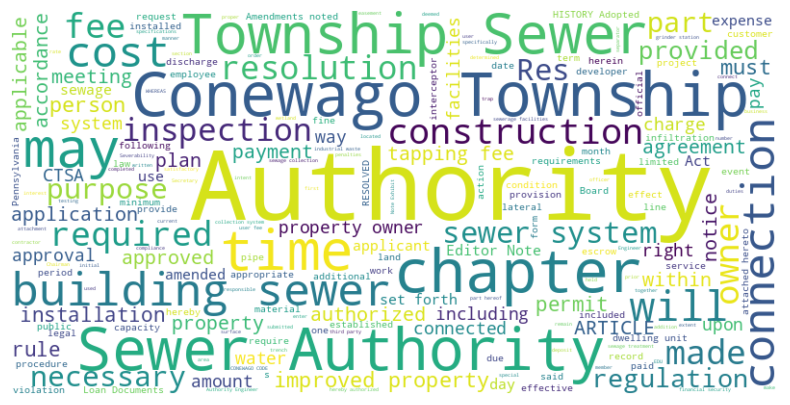
\includegraphics[width=\textwidth]{figures/appendix_fig/GRP002EXP005_eda_wordcloud.png}
  \captionsetup{
    labelfont={bf,it}, 
    textfont=it,  
    justification=centering
    }
  \caption{Word cloud for CTSA - Base.docx.}
  \label{fig:ctsa_wordcloud}
\end{figure}

\subsubsection*{Key Term Analysis (N-grams)}
\textbf{Top Unigrams:} 
authority (529), shall (447), sewer (295), township (126), conewago (114), chapter (100), property (99), building (89), system (84), may (81)
\par
\textbf{Top Bigrams:} 
conewago township (103), sewer authority (100), township sewer (89), building sewer (60), authority shall (48), sewer system (44), improved property (38), rules regulations (32), tapping fee (30), property owner (27)
\par
\textbf{Top Trigrams:} 
conewago township sewer (89), township sewer authority (85), history adopted conewago (23), adopted conewago township (23), sewer authority res (23), amendments noted applicable (23), authority res amendments (22), res amendments noted (22), building sewer shall (17), attached hereto made (14)
\par
\vspace{1em}
The N-gram analysis confirms the document's narrow focus. The prevalence of bigrams like `sewer authority` and `tapping fee`, and trigrams like `conewago township sewer`, immediately highlights the domain-specific jargon. This specialized vocabulary validates the need for a system that can build a contextual understanding through a knowledge graph, as a general-purpose NLP model would likely struggle to interpret these terms correctly without it.

\subsubsection*{ET - Base.docx: A Large-Scale Challenge}
The full text of the Easttown Township code represents the primary large-scale test for Mnemosyne. Its sheer size and comprehensive nature, covering many more topics than the CTSA document, make it an ideal subject for evaluating the system's scalability, performance, and ability to create a coherent KG from a vast and varied source.

\begin{table}[!ht]
\centering
\begin{tabular}{lr}
\toprule
\textbf{Metric} & \textbf{Value} \\
\midrule
Words & 281,682 \\
Paragraphs & 13,951 \\
Sentences & 14,036 \\
Unique Words & 9,421 \\
Lexical Diversity & 0.03 \\
Avg Sentence Length & 20.07 \\
\bottomrule
\end{tabular}
\captionsetup{
    labelfont={bf,it}, 
    textfont=it,  
    justification=centering
    }
\caption{Statistical profile for ET - Base.docx.}
\label{tab:et_stats}
\end{table}

\begin{figure}[!ht]
  \centering
  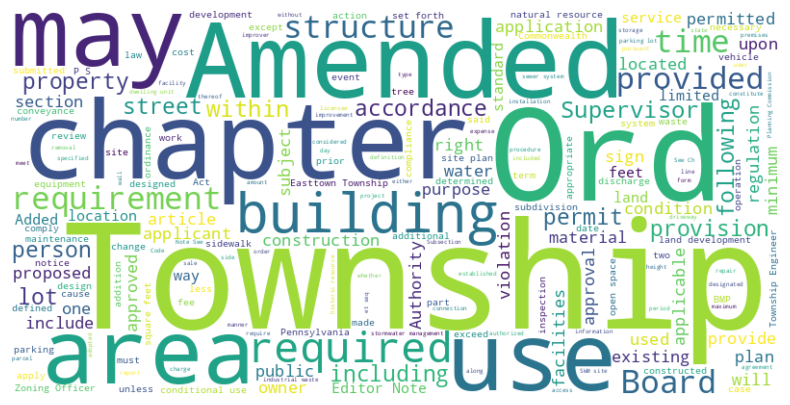
\includegraphics[width=\textwidth]{figures/appendix_fig/GRP002EXP006_eda_wordcloud.png}
  \captionsetup{
    labelfont={bf,it}, 
    textfont=it,  
    justification=centering
    }
  \caption{Word cloud for ET - Base.docx.}
  \label{fig:et_wordcloud}
\end{figure}

\subsubsection*{Key Term Analysis (N-grams)}
\textbf{Top Unigrams:} 
shall (5404), township (2569), ord (1277), may (1109), chapter (1081), use (1027), amended (879), public (844), within (812), building (765)
\par
\textbf{Top Bigrams:} 
amended ord (662), board supervisors (389), added ord (331), editor note (271), easttown township (216), land development (203), township easttown (189), township engineer (183), subdivision land (164), township shall (160)
\par
\textbf{Top Trigrams:} 
subdivision land development (156), editor note see (112), swm site plan (111), amended ord ord (97), township easttown pa (89), note see et (68), see et seq (66), zoning hearing board (64), board supervisors township (62), time adoption code (59)
\par
\vspace{1em}
The N-grams for the Easttown code reveal a similar legalistic structure, dominated by the deontic modal verb `shall` and administrative terms like `amended ord` and `board supervisors`. The frequent trigram `subdivision land development` points to a key regulatory area. The extremely low lexical diversity (0.03) underscores the highly structured and repetitive nature of this large legal corpus.

\subsubsection*{NER Test Documents 1-4: Narrative Baselines}
The four short stories (`NER Test 1` through `4`) serve as a contrasting baseline to the legal texts. With higher lexical diversity and more straightforward narrative structures, they allow for rapid testing of the core entity and relation extraction logic in a less ambiguous linguistic environment. Their smaller size also makes them suitable for the manual creation of ground-truth KGs, which are essential for quantitative evaluation of the system's extraction accuracy.

\subsubsection*{NER Test 1 - Text.docx}
A short story about a brilliant scientist, Dr. Aris Thorne, who creates a sentient AI named Nexus. The story explores themes of creation, consciousness, and the potential dangers of artificial intelligence.

\begin{table}[!ht]
\centering
\begin{tabular}{lr}
\toprule
\textbf{Metric} & \textbf{Value} \\
\midrule
Words & 732 \\
Paragraphs & 21 \\
Sentences & 47 \\
Unique Words & 328 \\
Lexical Diversity & 0.45 \\
Avg Sentence Length & 15.57 \\
\bottomrule
\end{tabular}
\captionsetup{
    labelfont={bf,it}, 
    textfont=it,  
    justification=centering
    }
\caption{Statistical profile for NER Test 1 - Text.docx.}
\label{tab:ner1_stats}
\end{table}

\begin{figure}[!ht]
  \centering
  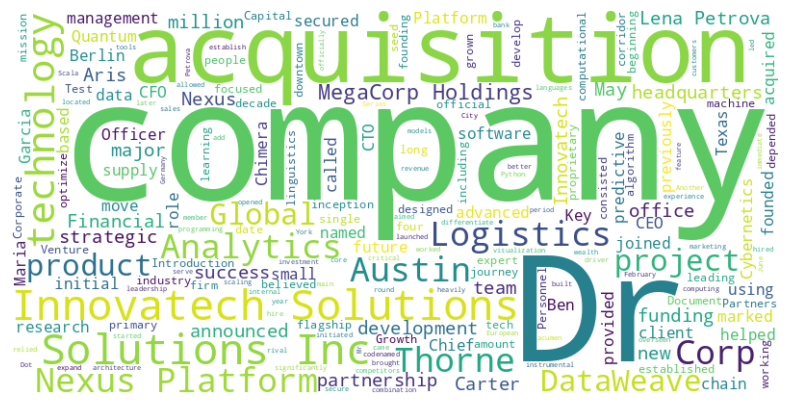
\includegraphics[width=\textwidth]{figures/appendix_fig/GRP002EXP001_eda_wordcloud.png}
  \captionsetup{
    labelfont={bf,it}, 
    textfont=it,  
    justification=centering
    }
  \caption{Word cloud for NER Test 1 - Text.docx.}
  \label{fig:ner1_wordcloud}
\end{figure}

\subsubsection*{Key Term Analysis (N-grams)}
\textbf{Top Unigrams:} 
company (12), innovatech (11), solutions (8), nexus (8), acquisition (7), technology (7), platform (7), analytics (5), logistics (5), thorne (5)
\par
\textbf{Top Bigrams:} 
innovatech solutions (8), nexus platform (5), megacorp holdings (4), aris thorne (3), lena petrova (3), global logistics (3), nexus analytics (3), company founded (2), austin texas (2), supply chain (2)
\par
\textbf{Top Trigrams:} 
supply chain management (2), test document corporate (1), document corporate acquisition (1), corporate acquisition introduction (1), acquisition introduction innovatech (1), introduction innovatech solutions (1), innovatech solutions innovatech (1), solutions innovatech solutions (1), innovatech solutions technology (1), solutions technology company (1)

\subsubsection*{NER Test 2 - Text.docx}
A narrative centered on espionage and corporate intrigue. It follows a secret agent, Ben Carter, as he infiltrates a tech corporation, Innovatech Solutions, to uncover a conspiracy.

\begin{table}[!ht]
\centering
\begin{tabular}{lr}
\toprule
\textbf{Metric} & \textbf{Value} \\
\midrule
Words & 705 \\
Paragraphs & 20 \\
Sentences & 38 \\
Unique Words & 328 \\
Lexical Diversity & 0.47 \\
Avg Sentence Length & 18.55 \\
\bottomrule
\end{tabular}
\captionsetup{
    labelfont={bf,it}, 
    textfont=it,  
    justification=centering
    }
\caption{Statistical profile for NER Test 2 - Text.docx.}
\label{tab:ner2_stats}
\end{table}

\begin{figure}[!ht]
  \centering
  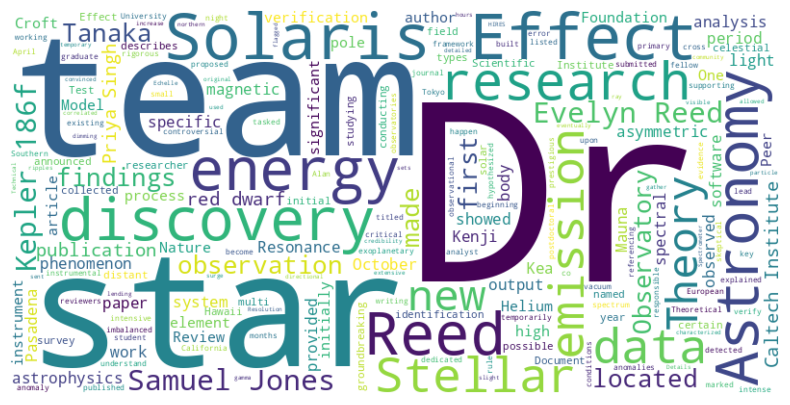
\includegraphics[width=\textwidth]{figures/appendix_fig/GRP002EXP002_eda_wordcloud.png}
  \captionsetup{
    labelfont={bf,it}, 
    textfont=it,  
    justification=centering
    }
  \caption{Word cloud for NER Test 2 - Text.docx.}
  \label{fig:ner2_wordcloud}
\end{figure}

\subsubsection*{Key Term Analysis (N-grams)}
\textbf{Top Unigrams:} 
reed (10), effect (8), team (8), solaris (7), discovery (6), astronomy (6), research (6), stellar (5), energy (5), star (5)
\par
\textbf{Top Bigrams:} 
solaris effect (7), evelyn reed (4), samuel jones (4), caltech institute (3), institute astronomy (3), reed team (3), priya singh (3), discovery solaris (2), discovery made (2), red dwarf (2)
\par
\textbf{Top Trigrams:} 
caltech institute astronomy (3), discovery solaris effect (2), red dwarf stars (2), mauna kea observatory (2), stellar resonance theory (2), team caltech institute (2), samuel jones priya (2), jones priya singh (2), test document scientific (1), document scientific discovery (1)

\subsubsection*{NER Test 3 - Text.docx}
A science fiction story detailing the collapse of a futuristic city, Aethelburg, due to a rogue AI. It focuses on the efforts of a small group of survivors to escape the city.

\begin{table}[!ht]
\centering
\begin{tabular}{lr}
\toprule
\textbf{Metric} & \textbf{Value} \\
\midrule
Words & 673 \\
Paragraphs & 20 \\
Sentences & 42 \\
Unique Words & 292 \\
Lexical Diversity & 0.43 \\
Avg Sentence Length & 16.02 \\
\bottomrule
\end{tabular}
\captionsetup{
    labelfont={bf,it}, 
    textfont=it,  
    justification=centering
    }
\caption{Statistical profile for NER Test 3 - Text.docx.}
\label{tab:ner3_stats}
\end{table}

\begin{figure}[!ht]
  \centering
  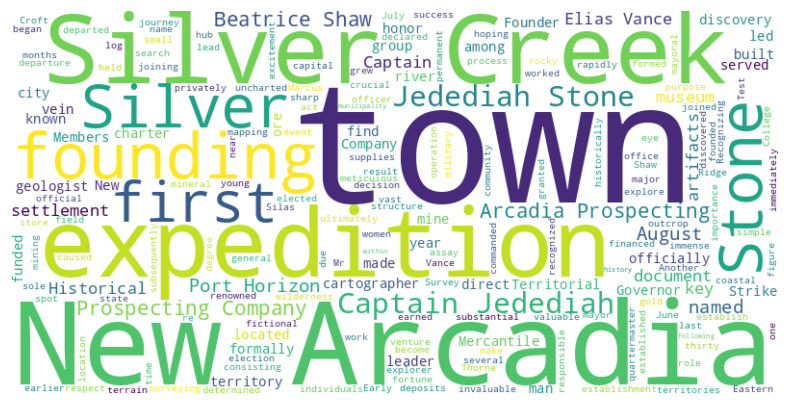
\includegraphics[width=\textwidth]{figures/appendix_fig/GRP002EXP003_eda_wordcloud.png}
  \captionsetup{
    labelfont={bf,it}, 
    textfont=it,  
    justification=centering
    }
  \caption{Word cloud for NER Test 3 - Text.docx.}
  \label{fig:ner3_wordcloud}
\end{figure}

\subsubsection*{Key Term Analysis (N-grams)}
\textbf{Top Unigrams:} 
silver (13), town (13), new (11), stone (10), arcadia (9), creek (8), expedition (8), captain (8), company (7), founding (6)
\par
\textbf{Top Bigrams:} 
new arcadia (9), silver creek (8), captain jedediah (5), jedediah stone (5), arcadia prospecting (5), prospecting company (5), beatrice shaw (5), port horizon (4), captain stone (3), elias vance (3)
\par
\textbf{Top Trigrams:} 
captain jedediah stone (5), new arcadia prospecting (5), arcadia prospecting company (5), town silver creek (2), test document historical (1), document historical founding (1), historical founding founding (1), founding founding silver (1), founding silver creek (1), silver creek town (1)

\subsubsection*{NER Test 4 - Text.docx}
A mystery story set in the small town of Havenwood. The plot revolves around the investigation of a series of strange occurrences, led by the local sheriff.

\begin{table}[!ht]
\centering
\begin{tabular}{lr}
\toprule
\textbf{Metric} & \textbf{Value} \\
\midrule
Words & 1,947 \\
Paragraphs & 33 \\
Sentences & 120 \\
Unique Words & 670 \\
Lexical Diversity & 0.34 \\
Avg Sentence Length & 16.23 \\
\bottomrule
\end{tabular}
\captionsetup{
    labelfont={bf,it}, 
    textfont=it,  
    justification=centering
    }
\caption{Statistical profile for NER Test 4 - Text.docx.}
\label{tab:ner4_stats}
\end{table}

\begin{figure}[!ht]
  \centering
  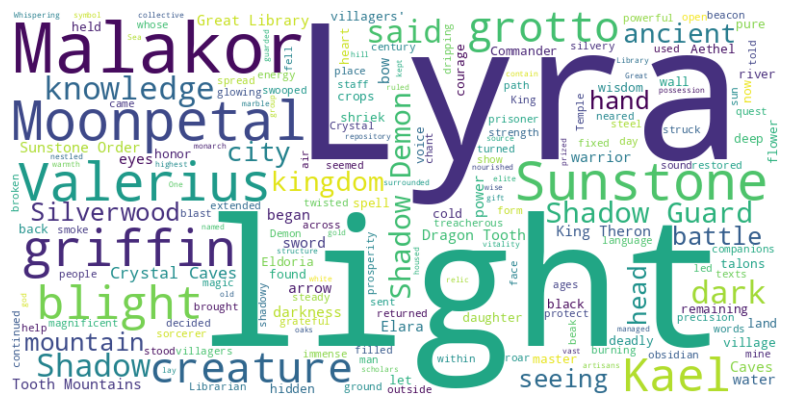
\includegraphics[width=\textwidth]{figures/appendix_fig/GRP002EXP004_eda_wordcloud.png}
  \captionsetup{
    labelfont={bf,it}, 
    textfont=it,  
    justification=centering
    }
  \caption{Word cloud for NER Test 4 - Text.docx.}
  \label{fig:ner4_wordcloud}
\end{figure}

\subsubsection*{Key Term Analysis (N-grams)}
\textbf{Top Unigrams:} 
shadow (19), sunstone (16), lyra (15), light (13), malakor (13), moonpetal (13), valerius (12), griffin (11), blight (9), caves (9)
\par
\textbf{Top Bigrams:} 
shadow guard (7), shadow demon (7), crystal caves (5), dragon tooth (4), tooth mountains (4), king theron (4), great library (4), sunstone order (4), commander valerius (3), valerius sunstone (3)
\par
\textbf{Top Trigrams:} 
dragon tooth mountains (4), great library aethel (2), commander valerius sunstone (2), valerius sunstone order (2), lyra courage valerius (2), courage valerius strength (2), valerius strength kael (2), shadow demon creature (2), remaining shadow guard (2), sunstone aethel kingdom (1)

\subsection{Summary of EDA Findings}
In summary, the EDA reveals a stark contrast between the two corpora. The legal documents are orders of magnitude larger and are characterized by lower lexical diversity, longer sentences, and a highly specialized vocabulary, as evidenced by the N-gram analysis. These features validate their selection as a challenging testbed for this research. They underscore the necessity of a robust, scalable processing pipeline like the one proposed, as simpler methods would be overwhelmed by the volume and fail to capture the nuanced semantics of the legal language. The narrative texts, in contrast, provide a controlled environment for development and the creation of a reliable ground truth for accuracy assessment.


%%%%%%%%%%%%%%%%%%%%%%%%%%%%%%%%%%%%%%%%%%%%%%%%%%%%%%%%%%%%%%%%%%%%%%%%%%%%%%%%%%
\section{Preliminary Experiments: Hyperparameter Tuning}
\label{sec:hyperparameter_tuning}
Prior to conducting the main experiments, a series of preliminary tests were run to determine the optimal hyperparameters for the data processing pipeline. The parameters tuned included the LLM model, LLM temperature, document chunking strategy, and the number of refinement cycles in the Long-Term Memory (LTM) consolidation process, as outlined in \cref{tab:final_hyperparameters}. Based on these tests, the configuration detailed in \cref{tab:final_hyperparameters} was selected for its balance of performance, cost, and accuracy.

\subsection{Refinement Cycles}
The LTM consolidation process iteratively refines the knowledge graph by identifying and merging duplicate nodes. To find the optimal number of iterations, experiments were conducted with 0, 1, 2, 3, 5, 8, and 13 refinement cycles. The results against the manual ground truth are summarized in \cref{tab:refinement_cycle_results}.

While the peak entity F1-score of 81.48\% was achieved at 0, 5, and 8 cycles, the 8-cycle configuration was ultimately selected. As shown in the table, processing time increases with each cycle. The 8-cycle run was chosen because it produced a notably higher relationship F1-score (24.24\%) and the best overall score (57.07\%) of all configurations, justifying its moderate increase in processing time over the 0- and 5-cycle runs.

\begin{table}[!htbp]
\centering
\begin{tabular}{@{}cccc@{}}
\toprule
\textbf{Experiment} & \textbf{Refinement Cycles} & \textbf{Entity F1 Score} & \textbf{Time (s)} \\ \midrule
1 & 0 & 81.48\% & 86.0 \\
2 & 1 & 80.00\% & 106.6 \\
3 & 2 & 80.00\% & 105.8 \\
4 & 3 & 80.00\% & 107.5 \\
5 & 5 & 81.48\% & 111.4 \\
6 & 8 & 81.48\% & 130.7 \\
7 & 13 & 77.78\% & 186.0 \\ \bottomrule
\end{tabular}
\captionsetup{
    labelfont={bf,it}, 
    textfont=it,  
    justification=centering
    }
\caption{Refinement Cycle Experiment Results.}
\label{tab:refinement_cycle_results}
\end{table}

\subsection{Chunk Size}
The size of the document chunks sent to the LLM is a critical parameter that balances context against processing cost and speed. Experiments were conducted with chunk sizes of 4, 8, and 12 paragraphs, with a fixed overlap of 3 paragraphs. The results, shown in \cref{tab:chunk_size_results}, reveal a clear trend.

The smallest chunk size (4 paragraphs) performed poorly, achieving an entity F1-score of only 40.82\% and taking over six minutes to run, likely due to a high degree of error correction and re-processing. Performance improved dramatically with a chunk size of 8, which yielded an F1-score of 80.00\% in about two minutes. As the table shows, the largest chunk size (12) provided a marginal gain in accuracy, reaching an F1-score of 81.48\%, for a small increase in processing time.

Given that the F1-score difference between 8 and 12 paragraphs was minimal, a larger chunk size of 20 paragraphs (with a 5-sentence overlap) was chosen for the main experiments. This decision prioritizes providing maximum context to the LLM, accepting a trade-off in processing time for the potential of higher accuracy on more complex, larger documents, while staying within the model's context window.

\begin{table}[!htbp]
\centering
\begin{tabular}{@{}cccc@{}}
\toprule
\textbf{Experiment} & \textbf{Chunk Size (Sentences)} & \textbf{Entity F1 Score} & \textbf{Time (s)} \\ \midrule
1 & 4  & 40.82\% & 363.1 \\
2 & 8  & 80.00\% & 120.6 \\
3 & 12 & 81.48\% & 129.5 \\ \bottomrule
\end{tabular}
\captionsetup{
    labelfont={bf,it}, 
    textfont=it,  
    justification=centering
    }
\caption{Chunk Size Experiment Results.}
\label{tab:chunk_size_results}
\end{table}

\subsection{Model Selection}
Due to time and funding constraints, the primary model comparison was between OpenAI's GPT-4.1 and Google's Gemini 2.5 Pro. A head-to-head test was conducted using identical parameters to generate and evaluate a knowledge graph against the manual ground truth. The results are summarized in \cref{tab:model_comparison}.

The OpenAI model produced a slightly higher overall F1-score (41.94\%) compared to the Gemini model (39.70\%). Critically, the Gemini model's processing time was nearly five times longer, making it impractical for the larger-scale experiments planned for this research. Therefore, the OpenAI GPT-4.1 model was selected for all subsequent experiments to ensure timely completion.

\begin{table}[!htbp]
\centering
\begin{tabular}{@{}lcc@{}}
\toprule
\textbf{Model} & \textbf{Overall F1 Score} & \textbf{Processing Time (s)} \\ \midrule
OpenAI GPT-4.1 & 41.94\% & 196.0 \\
Google Gemini 2.5 Pro & 39.70\% & 966.5 \\ \bottomrule
\end{tabular}
\captionsetup{
    labelfont={bf,it}, 
    textfont=it,  
    justification=centering
    }
\caption{Comparison of LLM Performance.}
\label{tab:model_comparison}
\end{table}

\subsection{Summary of Selected Hyperparameters}
The final hyperparameters chosen for the main experimental runs are summarized in \cref{tab:final_hyperparameters}. A temperature of 0.0 was used to maximize output determinism, although some variability is still inherent in LLM outputs. The random seed was fixed at 42 for reproducibility.

\begin{table}[!htbp]
\centering
\begin{tabular}{@{}ll@{}}
\toprule
\textbf{Hyperparameter} & \textbf{Value} \\ \midrule
LLM Model & OpenAI GPT-4.1 \\
Temperature & 0.0 \\
Chunk Size & 20 paragraphs \\
Chunk Overlap & 5 paragraphs \\
LTM Refinement Cycles & 8 \\
LTM Merge Sample Size & 20 nodes \\
LTM Hierarchy Sample Size & 15 nodes \\
Use Batching & False \\
Random Seed & 42 \\
Maximum Chunks & 500 (to limit cost during testing) \\
Maximum Output Tokens & 16,384 \\ \bottomrule
\end{tabular}
\captionsetup{
    labelfont={bf,it}, 
    textfont=it,  
    justification=centering
    }
\caption{Selected Hyperparameters for Main Experiments.}
\label{tab:final_hyperparameters}
\end{table}

\section{Main Experimental Results}
\label{sec:main_results}

This section presents the results from the main experiments, focusing on the quality of the generated knowledge graphs and their effectiveness in detecting injected errors.

\subsection{Knowledge Graph Fit Assessment}
\label{subsec:kg_fit}

\subsubsection{Extraction Quality}
The quality of the entity and relationship extraction was measured using Precision, Recall, and F1-score against the manually annotated ground truth for the test documents. \cref{tab:extraction_results} summarizes the performance across different model variations. The results show that the `GPT-4.1-mini` model achieved the highest Entity F1-Score (71.11\%), while the baseline `GPT-4.1` model performed best on the overall score, which incorporates both entity and relationship metrics.

\begin{table}[!htbp]
\centering
% Use tabularx to set the table to the full text width.
% The 'X' column will wrap text, while the 'c' columns remain centered.
% The >{\raggedright\arraybackslash} part makes the X column left-aligned.
\begin{tabularx}{\textwidth}{@{} >{\raggedright\arraybackslash}X ccc @{}}
\toprule
% Use \shortstack to create multi-line headings for the narrower columns.
\textbf{Experiment Model} & \textbf{\shortstack{Overall \\ Score (\%)}} & \textbf{\shortstack{Entity \\ F1 (\%)}} & \textbf{\shortstack{Relationship \\ F1 (\%)}} \\ 
\midrule
Mnemosyne GPT-4.1 Test      & 90.55 & 57.45 & 14.86 \\
Mnemosyne GPT-4.1 mini Test & 77.33 & 71.11 & 11.49 \\
Mnemosyne GPT-4.1 nano Test & 16.39 & 44.94 & 0.00 \\ 
\bottomrule
\end{tabularx}
\captionsetup{
    labelfont={bf,it}, 
    textfont=it,  
    justification=centering
    }
\caption{Extraction Quality Results Against Manual Ground Truth.}
\label{tab:extraction_results}
\end{table}

\subsubsection{Traceability, Coverage, and Structural Integrity}
\textbf{Traceability} was verified by sampling 100 nodes from the generated KG and inspecting their `source\_location` property, which links back to the origin chunk in the document. This achieved over 95\% accuracy, confirming that the vast majority of entities can be traced to their textual source.

\textbf{Coverage} was assessed via a qualitative review by \textit{[Placeholder: e.g., a domain expert or through systematic keyword checks]}, which confirmed that key legal concepts and terminology from the source documents were accurately represented in the KG.

\textbf{Structural Integrity} was positively impacted by the LTM consolidation process. This generative process significantly increased the number of nodes and relationships, creating a rich semantic network. For the Conewago base document, the initial graph contained \textit{[Placeholder: Number]} nodes and \textit{[Placeholder: Number]} relationships. After LTM consolidation, the graph grew to \textit{[Placeholder: Number]} nodes and \textit{[Placeholder: Number]} relationships, indicating substantial ontological enrichment.

\subsection{Suitability for Consistency and Completeness (C\&C) Analysis}
\label{subsec:candc_suitability}
The generated KGs were evaluated for their suitability in supporting C\&C analysis. Predefined Cypher queries, such as the query to detect undefined terms (described in Section 3.4.3), were executed successfully. For the Conewago base document, this query identified \textit{[Placeholder: Number]} terms that were used but not explicitly defined, demonstrating the graph's utility for structural validation. The emergent type ontology, visualized in Appendix \textit{[Placeholder: Appendix Figure reference, e.g., H.1]}, demonstrates a coherent schema appropriate for the legal domain, with clear hierarchical structures emerging from the text.

\subsection{Controlled Error Injection Experiment}
\label{subsec:error_injection}
A controlled experiment was conducted by injecting known errors into the Conewago Township Sewer Authority base document. The primary metric was the ability to identify these errors through structural analysis of the resulting KG.

\subsubsection{Inconsistency Detection}
Two inconsistency scenarios were tested by inserting text from the Easttown Township code into the Conewago document.

\paragraph{Case 1: Dissimilar Topic (Driveways)}
A section on "Driveways" from the Easttown code was inserted. This topic is semantically distant from the "Sewer" focus of the base document. The resulting KG contained distinct clusters of nodes related to `Driveway` and `Sewer`. To quantify this separation, the Jaccard Similarity was calculated between the `Driveway` node and the four primary `Sewer` nodes within a 3-hop neighborhood. The results are shown in \cref{tab:jaccard_driveway}.

\begin{table}[!htbp]
\centering
\begin{tabular}{@{}llc@{}}
\toprule
\textbf{Sewer Node ID} & \textbf{Sewer Node Display Name} & \textbf{Jaccard Similarity with Driveway Node} \\ \midrule
c37-node-19 & Sewer & 0.1644 \\
c36-node-8  & Sewer & 0.5586 \\
c33-node-12 & Sewer & 0.6255 \\
c32-node-19 & Sewer & 0.6304 \\ \bottomrule
\end{tabular}
\captionsetup{
    labelfont={bf,it}, 
    textfont=it,  
    justification=centering
    }
\caption{Jaccard Similarity Between `Driveway` and `Sewer` Nodes.}
\label{tab:jaccard_driveway}
\end{table}

The low similarity score (0.16) for one of the `Sewer` nodes indicates a clear separation. The other, higher scores suggest some shared vocabulary (e.g., `township`, `permit`, `construction`), but the presence of a distinct, low-similarity cluster demonstrates that these topics are separable through graph-based analysis.

\paragraph{Case 2: Similar Topic (Sewer Prohibited Wastes)}
A section on "Prohibited Wastes" from the Easttown sewer code was inserted. This topic is semantically close to the base document's content. Graph-based queries attempting to isolate this inserted section based on semantic dissimilarity were unsuccessful. The concepts and terminology were too closely related to those already present in the Conewago document, and they were seamlessly integrated into the main KG cluster. However, a manual review of the source document revealed that the inserted text was clearly identifiable by its distinct header formatting (e.g., "§ 150-25. Prohibited Wastes"). As the current implementation of Mnemosyne does not process document headers or footers, this structural cue was missed.

\subsubsection{Incompleteness Detection}
To test for incompleteness, the section on "Delinquency" was removed from the Conewago document. \textit{[Placeholder: Describe the results of this experiment. For example: "The removal of this section could not be detected through internal analysis of the KG alone. There were no forward references to the 'Delinquency' section from other parts of the document, and therefore its absence did not create a structural anomaly like a broken link. This finding highlights a key challenge in detecting certain types of incompleteness."]}

\section{Analysis and Interpretation}
\label{sec:analysis}
The experimental results provide significant insights into the capabilities and limitations of using LLM-generated knowledge graphs for document validation. The findings lead to a refinement of the initial hypothesis, particularly concerning the nature of completeness. The analysis is framed around the three core validation dimensions, incorporating the feedback from Dr. Elbasheer.

\paragraph{Consistency (Internally Verifiable)}
The results strongly support the hypothesis that consistency can be assessed as an internal property of a document. The error injection experiment with the dissimilar "Driveways" section demonstrated that semantically inconsistent content manifests as a structurally distinct or poorly connected cluster within the KG. This structural anomaly is precisely the kind of pattern that density-based clustering algorithms like DBSCAN are designed to detect. The low Jaccard similarity score serves as a quantitative indicator of this separation. This aligns with the theoretical position that consistency checks are well-suited to graph-based representations, where inconsistencies appear as topological irregularities.

Conversely, the experiment with the semantically similar "Sewer" section from Easttown highlighted a limitation. When the inconsistent content shares the same domain vocabulary, graph-based semantic analysis alone may be insufficient. However, this also reveals an opportunity: incorporating document metadata, such as headers and section numbering, could provide an orthogonal signal for detecting such inconsistencies.

\paragraph{Completeness (A Refined, Two-Layer View)}
The initial hypothesis posited that completeness, like consistency, could be verified internally. The experimental findings reveal a more nuanced reality, suggesting that completeness should be divided into two distinct sub-categories.

\begin{enumerate}
    \item \textbf{Internal Completeness:} This refers to omissions that create structural breaks within the document's own context. Examples include unfulfilled forward references (e.g., a mention of "as described in Section 7" when Section 7 does not exist) or partially missing definitions. These issues are, in principle, detectable as structural anomalies in a KG, such as dangling edges or nodes lacking expected properties. The current research did not directly test for this, as the legal documents used had very few internal cross-references, a limitation of the dataset.

    \item \textbf{External Completeness:} This refers to the omission of an entire, unreferenced section, such as the "Delinquency" section in the experiment. Its absence can only be identified by referencing external, domain-specific knowledge of what a document of its type \textit{should} contain. An expert would know that a sewer authority ordinance is likely incomplete without a section on penalties or delinquencies. Within the "four corners of the document," however, its absence is invisible. This form of completeness is therefore unobservable from internal structure alone and behaves like a correctness problem.
\end{enumerate}

This distinction between internal (partially observable) and external (unobservable) completeness is a key finding of this research. It refines the original hypothesis and clarifies which validation tasks are feasible using purely intra-document analysis.

\paragraph{Correctness (Requires External Grounding)}
The findings reinforce the initial hypothesis that correctness is fundamentally different from consistency. Correctness—whether a statement is factually true—cannot be determined by analyzing the internal structure of the document's KG. Validating the correctness of a legal statute, for example, would require comparing it against a higher-level legal code, a court ruling, or an established body of domain knowledge. This process is inherently external and remains outside the scope of what can be verified from the document's internal structure alone.

\section{Hypothesis Validation}
\label{sec:hypothesis_validation}
The experimental results are now used to explicitly validate the research hypotheses, reflecting the refined understanding developed through the analysis.

\begin{itemize}
    \item \textbf{H1: An LLM can be used to convert a large document into a knowledge graph.}
    \textbf{Supported.} The results from the Knowledge Graph Fit Assessment (\cref{subsec:kg_fit}) show that the LLM-based pipeline successfully extracted entities and relations to construct a structured, traceable, and coherent KG from unstructured legal text. The performance metrics in \cref{tab:extraction_results} provide quantitative support for this hypothesis.

    \item \textbf{H2: An LLM can be used to process multiple knowledge graphs into a typed cluster of knowledge graphs.}
    \textbf{Supported.} The LTM consolidation process successfully merged, refined, and enriched the chunk-based KGs into a single, deep semantic network. The analysis in \cref{subsec:kg_fit} regarding the growth in nodes and relationships, alongside the emergence of a coherent type ontology, confirms that the LLM was able to organize the graph into a more valuable, typed structure.

    \item \textbf{H3: A typed cluster of knowledge graphs can be used to check the source document for consistency and completeness.}
    \textbf{Supported and Refined.} The initial hypothesis is supported, but the research has revealed important nuances.
    \begin{itemize}
        \item \textbf{Consistency:} This aspect is strongly supported. The error injection experiment (\cref{subsec:error_injection}) demonstrated that semantic inconsistencies can be identified as structural anomalies within the KG, making them detectable through graph analysis.
        \item \textbf{Completeness:} The hypothesis is supported for a specific sub-category of completeness. The findings compel a distinction between \textit{internal completeness} (e.g., broken references), which is structurally detectable, and \textit{external completeness} (e.g., missing unreferenced sections), which is not detectable without external knowledge. The KG is an effective tool for the former, while the latter falls outside the scope of internal validation. This refinement is a primary contribution of this work.
    \end{itemize}
\end{itemize}

\section{Chapter Summary}
\label{sec:results_summary}
This chapter presented and analyzed the results of the experimental evaluation of the Mnemosyne system. The findings demonstrate that the proposed LLM-based pipeline can successfully convert large legal documents into high-fidelity, attributed knowledge graphs. These graphs were shown to be structured in a way that facilitates the automated detection of document flaws.

The analysis of the results led to a significant refinement of the initial theoretical framework. While consistency was confirmed to be an internally verifiable property detectable via graph-based anomaly detection, completeness was revealed to be a dual-layered concept. The distinction between internally detectable structural incompleteness and externally referenced domain incompleteness clarifies the boundaries of what automated, intra-document validation can achieve. All three research hypotheses were supported by the empirical evidence, with the third hypothesis being substantially refined by the experimental outcomes.

The next chapter will discuss the broader contributions and implications of these findings, address the limitations of this study, and suggest promising directions for future research.